%!TEX root = ../../Heun_Dale_Haney_A_dynamic_approach_to_input_output_modeling.tex
%%%%%%%%%%%%%%%%%%%%% chapter.tex %%%%%%%%%%%%%%%%%%%%%%%%%%%%%%%%%
%
% sample chapter
%
% Use this file as a template for your own input.
%
%%%%%%%%%%%%%%%%%%%%%%%% Springer-Verlag %%%%%%%%%%%%%%%%%%%%%%%%%%
%\motto{Use the template \emph{chapter.tex} to style the various elements of your chapter content.}
\motto{Accounting systems change behavior.

\hfill---\emph{unknown NASA JPL accountant}}

%%%%%%%%%%%%%%%%%%%%%%%%%%%%%%%%%%%%%%
%%%%%%%%%% Energy Intensity %%%%%%%%%%
%%%%%%%%%%%%%%%%%%%%%%%%%%%%%%%%%%%%%%
\chapter{Energy intensity}
% Always give a unique label
\label{chap:intensity} 
% use \chaptermark{} to alter or adjust the chapter heading in the running head
\chaptermark{Intensity}
%%%%%%%%%%%%%%%%%%%%%%%%%%%%%%%%%%
%%%%%%%%%%%%%%%%%%%%%%%%%%%%%%%%%%
%%%%%%%%%%%%%%%%%%%%%%%%%%%%%%%%%%

%% \abstract{Each chapter should be preceded by an abstract (10--15 lines long) that summarizes the content. The abstract will appear \textit{online} at \url{www.SpringerLink.com} and be available with unrestricted access. This allows unregistered users to read the abstract as a teaser for the complete chapter. As a general rule the abstracts will not appear in the printed version of your book unless it is the style of your particular book or that of the series to which your book belongs.\newline\indent
%% Please use the 'starred' version of the new Springer \texttt{abstract} command for typesetting the text of the online abstracts (cf. source file of this chapter template \texttt{abstract}) and include them with the source files of your manuscript. Use the plain \texttt{abstract} command if the abstract is also to appear in the printed version of the book.}

%% Use the template \emph{chapter.tex} together with the Springer document class SVMono (monograph-type books) or SVMult (edited books) to style the various elements of your chapter content in the Springer layout.

\abstract*{In this chapter, we derive algebraic equations that describe the energy intensity
(in units of J/\$) of products of economic sectors.
The algebraic equations are applied 
to Examples~A--C to derive a matrix equation % chktex 8
for a vector of energy intensities for the entire economy.
We review several studies of energy intensity in the literature 
and note a wide range of results from one study to the next.
The estimates of energy intensity also vary with time.
The range of energy intensities for the auto sector 
is $0.83 \times 10^{4}$ kJ/\$ to $11.6 \times 10^{4}$ kJ/\$.}

At the end of Chapter~\ref{chap:intro}, 
we noted that in the age of resource depletion,
routine dissemination of information regarding
energy, embodied energy, and energy intensity would
provide firms and consumers with better information to
navigate upcoming energy transitions.
To that end, we developed equations that describe the
flow and accumulation of direct energy, embodied energy, and economic value within an economy
in Chapters~\ref{chap:direct_energy},~\ref{chap:embodied_energy}, and~\ref{chap:value}.
In this chapter, we merge energy and economic value together to estimate
the energy intensity ($\varepsilon$) of economic sectors,
measured in joules per dollar.%
	\footnote{
	The literature discusses 
	the energy embodied in \emph{products} for example, 
	``The data and methodologies described in this report 
	permit calculation of five types of energy `embodied' 
	in a particular goods~[\emph{sic}] or service.''~\cite[p.~268]{Bullard:1978vd} % chktex 38
	It can be meaningful to discuss the energy intensity of \emph{processes}, too,
	and we switch between these two meanings of the word ``embodied.''
	}


%%%%%%%%%% Background %%%%%%%%%%
\section{Background}
\label{sec:IO_background}
%%%%%%%%%%

Input-Output (I-O) analysis, developed by Wassilly Leontief in the 1930s 
as an extension to the work of Quesnay and Walras~\cite{Leontief1936}, 
is of primary importance in national accounting. 
The method allows determination of the flows of value through
an economy as well as, 
among other things, 
calculation of a nation's gross domestic product (GDP), 
today's prevailing measure of economic activity.

The basic premise of the I-O method, 
as depicted in Figure~\ref{fig:basic_unit}A, 
is that each economic sector takes in factors of production 
from other sectors (and possibly itself) 
to produce an economic good at some rate.%
	\footnote{
	Note that Figure~\ref{fig:basic_unit}A is similar to the 
	clockwork metaphor and traditional model of the economy discussed
	in relation to the era of abundance in Section~\ref{sec:era_of_abundance}.
	}
For example, the automotive sector takes in steel, rubber, glass, etc. 
and produces a number of cars per year. 
In contrast to high-level economic growth models 
that include only a few factors of production (such as land, capital, and labor),%
	 \footnote{
	 The traditional primary factors of production (land, capital, and labor) 
	 are not \emph{flows} into the production processes. 
	 Rather, they are \emph{stocks} that, when present, 
	 allow factors of production (steel, rubber, and glass) 
	 to be transformed into final products (automobiles). 
	 The quantity and quality of these stocks 
	 determine the quantity and quality of their flow of productive services.
	 }
the I-O analysis technique allows many differentiated factors of production 
and raw material feedstocks.\cite{Costanza:1980ww} 
This is important, because, in reality, 
each economic process exists in a complex network of
interacting processes that comprise the entire economy.
Bullard et al.\ said 
``each step in a process analysis may be viewed as 
an expansion of the system boundary 
(around the item being analyzed) 
into the economic system.''~\cite[p.~281]{Bullard:1978vd}
Figure~\ref{fig:Hybrid_boundary} shows that 
every process calls on every other process within the economy,
even if only minutely and indirectly at many steps removed.

\begin{figure}[!ht]
\centering\
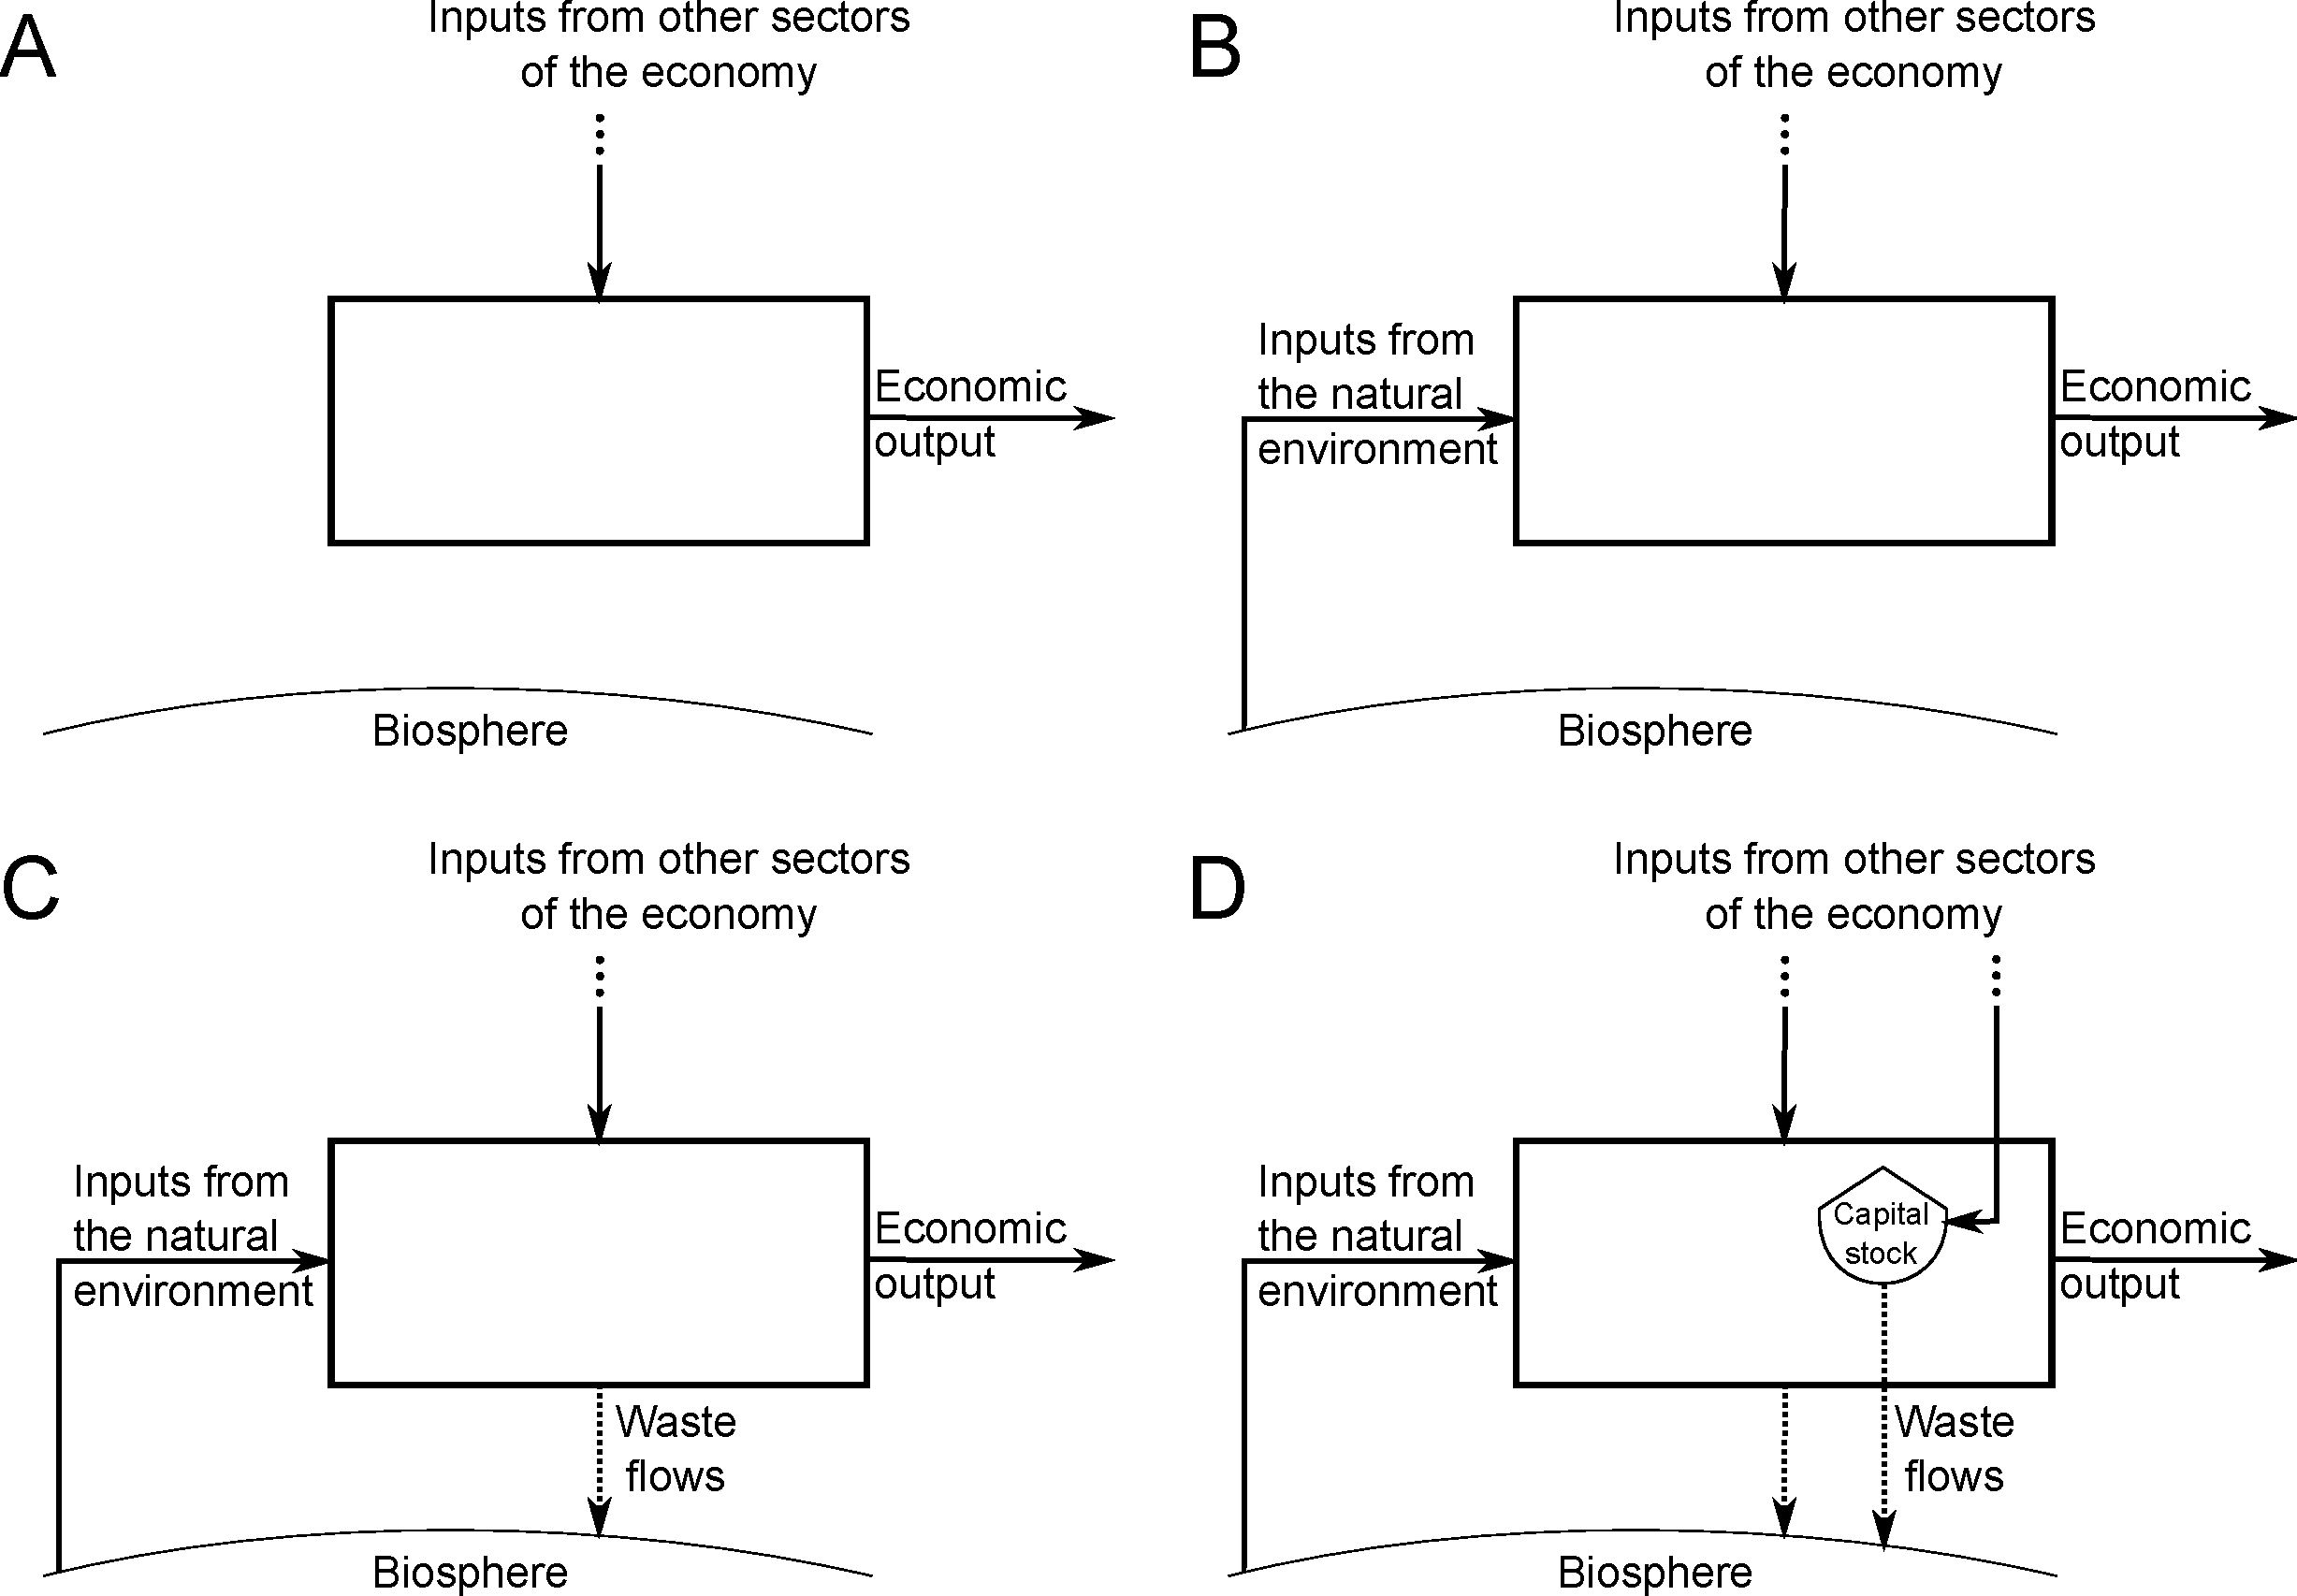
\includegraphics[width=\linewidth]{Part_2/Chapter_Intensity/images/Basic_unit_square.pdf}
\caption[The basic unit of input-output analysis]{The basic unit 
of input-output analysis: 
\textbf{A} the standard economic approach includes only transactions 
among sectors of the economy; 
\textbf{B} the Energy Input-Output (EI-O) method allows inputs 
from the natural environment to be factors of production; 
\textbf{C} including waste flows to the environment makes the model physically consistent; and
\textbf{D} the framework developed and presented herein accounts also for accumulation
in capital stock ($K$) of embodied energy within materials in economic sectors.}
\label{fig:basic_unit}
\end{figure}

\begin{figure}[p]
\centering\
\includegraphics[width=\linewidth]{Part_3/Chapter_Unfinished/images/Hybrid_boundary.pdf}
\caption[System boundary for process and I-O analyses]{System boundary for process and I-O analyses, adapted from~\cite{Bullard:1978vd}.}
\label{fig:Hybrid_boundary}
\end{figure}

As discussed in Chapter~\ref{chap:acct_for_won}, 
the oil shocks of the 1970's spurred great interest in
the important role of energy in economic production.
In addition to the productive services 
provided by stocks of capital and labor,
a flow of energy%
	\footnote{
	Or, more precisely, 
	the degradation of an exergetic gradient/destruction of exergy.
	} 
is required for economic activity. 
These energy flows originate from the biosphere, 
recognition of which prompted researchers from the field of 
Net Energy Analysis (NEA) to extend 
the traditional Leontief
input-output method to include important 
energy flows from the environment, 
developing an Energy Input-Output (EI-O)
method as depicted in Figure~\ref{fig:basic_unit}B.%
	\footnote{
	Note that Figure~\ref{fig:basic_unit}B is similar to the 
	machine metaphor and engine model from the era of energy constraints
	discussed in Section~\ref{sec:era_of_energy_constraints}.
	}
\cite{Carter1974,
Bullard1975,Bullard1976a,Herendeen1978,Costanza:1980ww,
Casler1984,Joshi:1999uw,Suh2009}
While the Leontief input-output method
relies exclusively 
on monetary units to represent value flows 
among sectors of an economy, 
EI-O method 
relies upon physical units 
(especially energy units of joules) 
to represent some of the flows among economic sectors. 
In doing so, 
energy intensities ($\varepsilon$) of product flows can be estimated. 

What counts for energy input to a sector of the economy 
is an issue that must be considered.
The early pioneers of the EI-O method
counted only post-solar energy inputs to the economy, 
in a manner similar to our approach as discussed 
in the introduction to Chapter~\ref{chap:embodied_energy}.
About a decade later, Costanza~\cite{Costanza:1978vd} 
included an option to consider 
solar energy as an input to the economy, 
thereby significantly increasing the energy intensity 
of agricultural sectors and other sectors 
that depend upon agricultural outputs. 
However later work by Costanza~\cite{Costanza:1980ww, Costanza:1984tq} 
did not include solar input to the economy.

Whether solar input to the economy 
should be considered in a materials, energy, and economic value 
accounting framework is probably dependent upon 
the objectives of the analysis. 
The motivation for this particular book is primarily 
the effects of declining energy natural resource quality
on industrialized economies in the age of resource depletion. 
As such, inclusion of solar flows is probably unnecessary. 
However, expanding the framework to include non-industrialized 
or agrarian societies may require accounting for solar energy flows.%
	\footnote{
	In our framework, solar energy flows could be accounted as short-term ($\dot{S}$) flows
	for agricultural and forestry sectors
	and for
	solar thermal, 
	solar photovoltaic, 
	wind, 
	ocean thermal, 
	hydro, and
	biomass
	renewable energy
	production sectors.
	Doing so would not account for longer-term storage
	of solar energy used to form fossil fuels, 
	but fossil fuels are already accounted by the energy input vector ($\vec{E}_{0}$)
	in the framework presented in this book.
	See the introduction to Chapter~\ref{chap:embodied_energy} for a short discussion
	of another approach: emergy.
	}

The early EI-O method assumes that 
each economic sector makes a single product ($\dot{P}$).\cite{Bullard-III:1975aa}
In later years, the EI-O method was extended 
in the literature to include
co-products for each economic sector.\cite{Costanza:1984tq,Casler1984} 
To do so, both \emph{make} and \emph{use} data must be employed.%
	\footnote{
	The \emph{make-use} method is sometimes also called the
	\emph{supply-use} method.
	}
For the purposes of simplicity, 
we decided to leverage the older,
single-product formulation of the EI-O method.
The materials, energy, and value accounting framework
presented herein is more easily understood 
without the additional complexity of the make-use formulation 
of the EI-O method.
Recent work has shown that converting between the two forms of the I-O method
is possible.\cite{Soklis:2009aa}

The EI-O method can be considered a ``top-down'' analysis approach for
estimating energy intensity.
An alternative, ``bottom-up'' approach, 
that we will discuss here briefly but not employ in this book,
consists of detailed, process-based analysis
of specific economic processes.
Process analysis calculates the
energetic and material flows associated with the process
under study by disaggregating the process into
several components or sub-processes.
Model specification and data collection for process analysis is arduous,
time-consuming,
and costly.
Obviously,
the time, 
effort,
and cost involved with trying to model and
measure all of the flows in process analysis becomes daunting
for even low numbers of interacting processes.
The decision of where to draw the boundary of
a process analysis is known in the 
lifecycle assessment literature as the 
\emph{truncation problem}.\cite{Suh2004}
A comparison of the top-down and bottom-up approaches is provided 
in Figure~\ref{fig:IO_vs_process}.
For the purposes simplicity,
we focus on top-down EI-O methods in this book.%
	\footnote{
	It is possible to pursue hybrid top-down and bottom-up analysis methods.
	They hybrid approach 
	utilizes data from an EI-O analysis to supplement the
	missing data from truncation of a process analysis.
	The financial cost of goods and services identified by
	the process analysis are converted to energy
	(or material) flows via the EI-O method.
	The truncation error is replaced by a smaller aggregation
	error due to limitations of the EI-O 
	method.\cite{Bullard:1978vd}
	A variety of other hybrid methods exist which also aim to
	overcome the limitations of either process or I-O method 
	individually.\cite{Bullard:1978vd, Suh2004, Suh2002, 
	Crawford2008, Zhai2010}	
	}

\begin{figure}[p]
\centering\
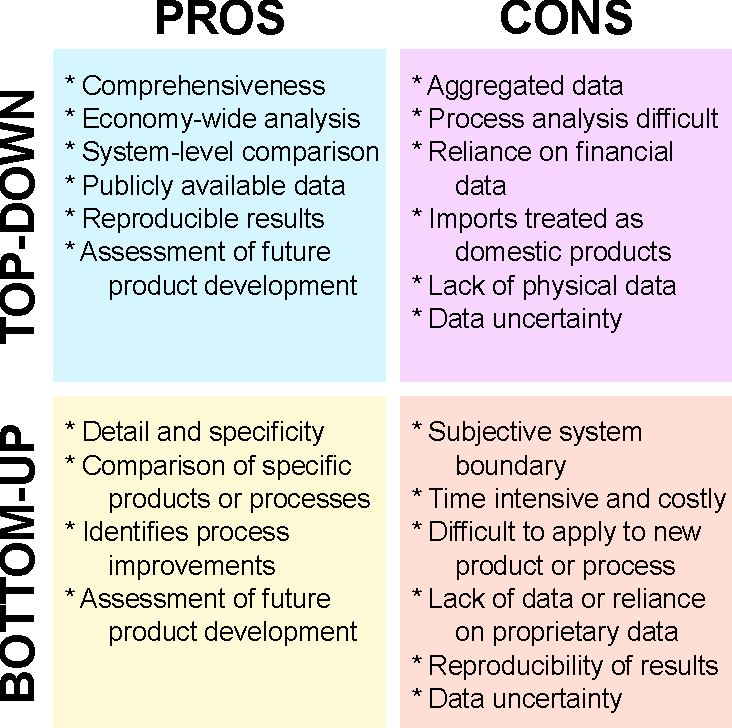
\includegraphics[width=0.8\linewidth]{Part_3/Chapter_Unfinished/images/Top_down_vs_bottom_up.pdf}
\caption[Top-down vs.\ bottom-up analyses]{Advantages (pros) and disadvantages (cons) of ``top-down,'' I-O and ``bottom-up,'' process-based analyses.
Adapted from~\cite{Hendrickson2006}.} % chktex 38
\label{fig:IO_vs_process}
\end{figure}

Both the original Leontief input-output method
(Figure~\ref{fig:basic_unit}A)
and the EI-O extension cited above
(Figure~\ref{fig:basic_unit}B)
assume steady-state conditions in an economy, 
i.e., flows of economic value and material into 
and out of each economic sector are in balance.
Wastes are not present, and
dynamic or transient behavior 
of the economic system is not considered. 
Thus, in the EI-O analysis technique, 
there is no accumulation of economic factors
or embodied energy
within any of the sectors. 

The EI-O approach provides ``snapshots'' 
of economic activity at an instant in time,
but its model is incomplete.
Figures~\ref{fig:basic_unit}C and~D show that wastes exist and
materials can accumulate in economic sectors as manufactured capital.%
	\footnote{
	Note that Figures~\ref{fig:basic_unit}C and~D are similar to the 
	metabolic metaphor that we propose for the age of resource depletion
	as discussed in Section~\ref{sec:age_of_resource_depletion}.
	}
In fact, assuming no accumulation of materials, 
within economic sectors or society itself, 
is tantamount to assuming that \emph{all} material flows 
through the economy are directed toward 
the production of non-durable goods. 
However, evidence of the durability of goods 
and the accumulation of materials surrounds us. 
Furthermore, 
energy was required to both fabricate and emplace 
the durable goods and infrastructure of modern economies.% 
	\footnote{
	The energy it took to create and emplace durable goods and infrastructure 
	can be considered ``embodied'' within the built environment, 
	a point to which we will return in detail later.
	}
As Georgescu-Roegen notes, 
``in the everyday world one cannot possibly cross a river 
only on the flow of maintenance materials 
of a non-existent bridge.''~\cite{G-R1975}

Because economic activity requires energy, 
we need to understand the way energy flows through economies. 
The steady-state EI-O techniques of Bullard, Herendeen, 
and others~\cite{Bullard1975,Herendeen1978} 
offer a starting point to that end. 
But, we need to move toward a fuller picture of 
the role of energy and manufactured capital in the economy;
we need to move toward Figures~\ref{fig:basic_unit}C and~D.
In the sections below, we utilize the
the results from
Chapters~\ref{chap:materials}--\ref{chap:value}
and extend the steady-state EI-O
techniques to estimate energy intensity given the existence of
wastes and the accumulation of embodied energy.


%%%%%%%%%% Methodology %%%%%%%%%%
\section{Methodology}
%%%%%%%%%%

Energy intensity ($\varepsilon$)
is the ratio 
of total energy ($\dot{T}$) 
and value ($\dot{X}$) outflow rates 
from an economic sector (e.g., the auto industry), 
such that for sector $j$,
%
\begin{equation} \label{eq:epsilon_output_def_g_and_s}
	\varepsilon_{j} \equiv \frac{\dot{T}_{j}}{\dot{X}_{j}},
\end{equation} 
%
and $\varepsilon$ is in units of J/\$.\footnote{It may be
instructive to consider energy intensity as the quotient
of embodied energy (in units of J/kg) and price (in \$/kg).}
Energy intensity ($\varepsilon_j$) represents the total energy demanded
by sector~$j$ (both for sector~$j$ itself and the energy required to
create the inputs to sector~$j$) per dollar of output from sector $j$.
Equation~\ref{eq:epsilon_output_def_g_and_s}
includes the embodied energy of products in the numerator ($\dot{T}_{j}$) term. 
A narrower definition ef energy intensity would be 
$\varepsilon_{j}~\equiv~\frac{\dot{Q}_{j0}}{\dot{X}_{j}}$,
which includes only energy consumed by sector $j$
in the numerator
and excludes the energy demanded upstream by the 
resource flows ($\dot{R}$) that comprise the product of the sector ($\dot{P}$).
We choose the broader definition of
Equation~\ref{eq:epsilon_output_def_g_and_s},
because it accounts for upstream energy consumption,
thereby providing an estimate of the true total energy cost of products.

For inter-sector flows, we have
%
\begin{equation} \label{eq:epsilon_transfers_1}
	\varepsilon_{j} = \frac{\dot{T}_{jk}}{\dot{X}_{jk}}.
\end{equation}
%
for all $k$, because the energy intensity 
of output from sector $j$ is independent of its destination ($k$). 
In other words, all goods produced by a sector 
are produced at the average energy intensity 
of that sector.\footnote{If this approach is unsatisfactory, 
the sector may be divided into sub-sectors 
each with its own energy intensity.}

We define the input-output ratio~($a_{ij}$)
that represents the input 
of good $i$ required to produce a unit of output from sector $j$.
%
\begin{equation} \label{eq:aij_def}
	a_{ij} \equiv \frac{\dot{X}_{ij}}{\dot{X}_{j}}
\end{equation}

We note that the value ($\dot{X}$) of all material flows must be counted such that
%
\begin{equation} \label{eq:aij_def_expanded}
	a_{ij} =	 
	\frac{\dot{X}_{\dot{R}_{ij}} + \dot{X}_{\dot{S}_{ij}} + \dot{X}_{\dot{K}_{ij}}}
		{\dot{X}_{\dot{R}_{j}} + \dot{X}_{\dot{S}_{j}} + \dot{X}_{\dot{K}_{j}}}.
\end{equation}
%
where $R$ represents resources,
$S$ represents short-lived materials, and
$K$ represents capital,
as discussed in Chapter~\ref{chap:materials}.

Input-output ratios~($a_{ij}$) are given in mixed units, 
depending on both the purpose of each sector of the economy 
and the type of input as shown in Figure~\ref{fig:A_matrix_units}.

\begin{figure}[ht!]
\centering\
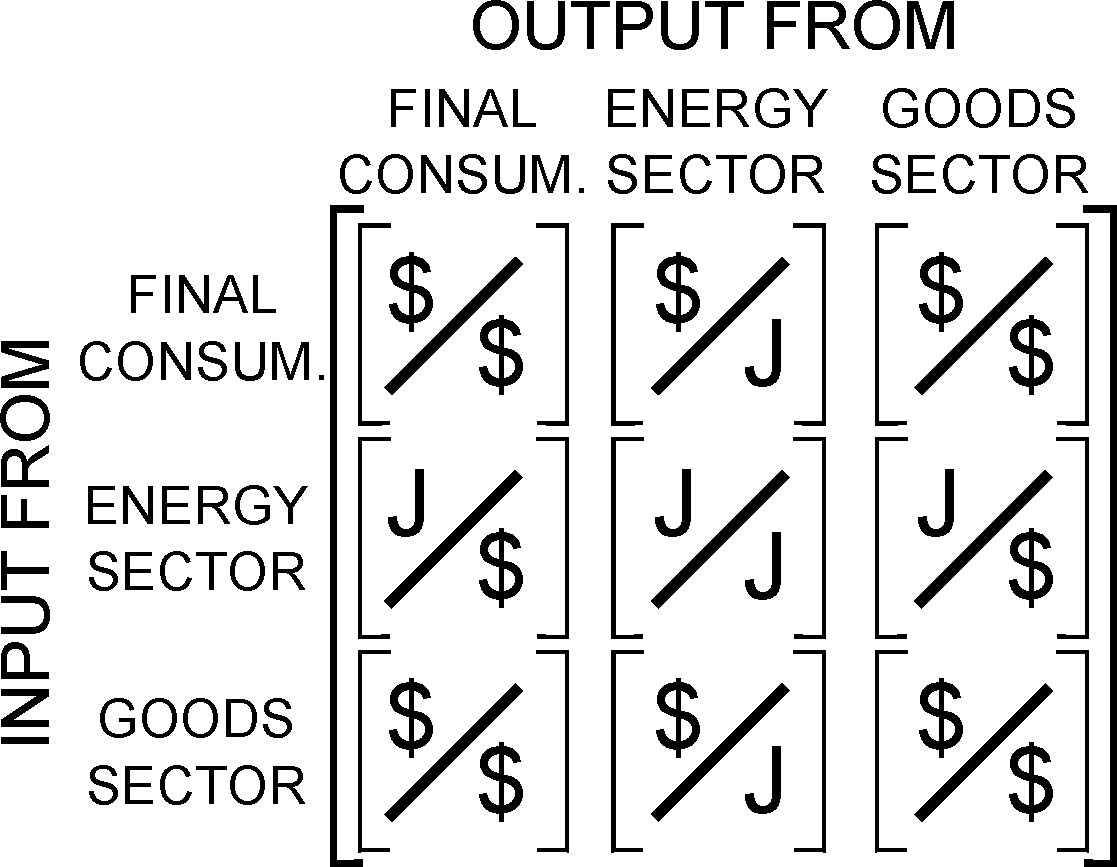
\includegraphics[width=0.4\linewidth]{Part_2/Chapter_Intensity/images/I-O_units.pdf}
\caption[Units for input-output ratios]{Units for input-output 
ratios~($a$).}
\label{fig:A_matrix_units}
\end{figure}

Equations~\ref{eq:epsilon_transfers_1} and~\ref{eq:aij_def} can be combined to give
%
\begin{equation}
	\dot{T}_{jk} = \varepsilon_{j} a_{jk} \dot{X}_{k}.
\end{equation}
%
That is,
the flow of total energy from sector $j$ into sector $k$~($\dot{T}_{jk}$),
is given by the energy intensity of sector $k$~($\varepsilon_{j}$)
multiplied by the amount of input good $j$ is required 
to produce a unit of output from sector $k$~($a_{jk}$)
multiplied by the output flow of value from sector $k$~($\dot{X}_{k}$).


%%%%%%%%%% Example A %%%%%%%%%%
\section{Example~A: single-sector economy} % chktex 13
%%%%%%%%%%

With reference to Figures~\ref{fig:A_energy}, 
\ref{fig:A_total_energy_T_dot}, 
and~\ref{fig:A_value},
the energy intensity ($\varepsilon_{1}$) of a single-sector economy is calculated by
%
\begin{equation} \label{eq:A-energy_intensity}
	\varepsilon_{1} 
	= \frac{\dot{T}_{1}}{\dot{X}_{1}} 
	= \frac{\dot{T}_{11}}{\dot{X}_{11}}.
\end{equation}

Appendix~\ref{chap:infinite_series} illustrates that the energy 
intensity of a single-sector economy ($\varepsilon_{1}$) 
is comprised of the sum of the infinite recursions
of energy consumed during production of output ($\dot{X}_{1}$).

To estimate energy intensities
when more than one economic sector is involved, 
we move to Examples~B and~C in the following sections.


%%%%%%%%%% Example B %%%%%%%%%%
\section{Example~B: two-sector economy} % chktex 13
%%%%%%%%%%

With reference to Figures~\ref{fig:B_energy}, 
\ref{fig:B_total_energy},
and~\ref{fig:B_value}, 
the energy intensity ($\varepsilon_{2}$) 
of the production sector is given by
%
\begin{equation} \label{eq:single_sector_energy_intensity}
	\varepsilon_{2} 
	= \frac{\dot{T}_{2}}{\dot{X}_{2}} 
	= \frac{\dot{T}_{22}}{\dot{X}_{22}}.
\end{equation}
%
Thus,
%
\begin{equation} \label{eq:T_dot_1_single_sector}
	\dot{T}_{2} = \varepsilon_{2}\dot{X}_{2},
\end{equation}

The input-output ratio 
for the production sector's self-use of output ($a_{22}$) is
%
\begin{equation} \label{eq:io_ratio_single_sector}
	a_{22} = \frac{\dot{X}_{22}}{\dot{X}_{2}},
\end{equation}
%
thus
%
\begin{equation} \label{eq:T_dot_11_single_sector}
	\dot{T}_{22} = \varepsilon_{2}a_{22}\dot{X}_{2}.
\end{equation}

We can rewrite the total energy accounting equation 
for Production~(2)
%
\begin{equation}
	\frac{\mathrm{d}T_{2}}{\mathrm{d}t} 	 
	= \dot{T}_{02} 
	+ \dot{T}_{12}
	+ \dot{T}_{22} 
	- \dot{T}_{2} 
	- \dot{T}_{20} \tag{\ref{eq:CV_T_2}}
\end{equation}
%
using energy intensity by realizing that:
%
\begin{itemize}
	\item{$\frac{\mathrm{d}E_2}{\mathrm{d}t} = 0$
		meaning that
		$\frac{\mathrm{d}T_2}{\mathrm{d}t} = \frac{\mathrm{d}B_2}{\mathrm{d}t}$, 
		because direct energy
		does not accumulate within economic sectors,}
	\item{$\frac{\mathrm{d}B_2}{\mathrm{d}t} = \frac{\mathrm{d}B_{K_{2}}}{\mathrm{d}t}$,
		because resources ($R$) and short-lived materials ($S$) do not 
		accumulate at appreciable rates in economic sectors,}
	\item{$\dot{B}_{02} = 0$ meaning that $\dot{T}_{02} = \dot{E}_{02}$,
		because flows from the biosphere have yet to have any energy from society embodied in them,}
	\item{$\dot{E}_{20} = 0$ meaning that $\dot{T}_{20} = \dot{B}_{20}$, 
		because direct energy is not wasted to the biosphere at any significant rate,%
			\footnote{Oil spills and gas leaks notwithstanding. 
			Remember also that waste heat outflows ($\dot{Q}_{20}$)
			are allocated to the product.
			} 
		and} 
	\item{$\dot{B}_{20} = \left( \dot{B}_{\dot{R}_{20}} 
							+ \dot{B}_{\dot{S}_{20}}
							+ \dot{B}_{\dot{K}_{20}}
							\right)
						= \left( \dot{B}_{\dot{R}_{20}} 
							+ \dot{B}_{\dot{S}_{20}}
							+ \gamma_{B_{2}} B_{K_{2}}
							\right)$, as shown in Section~\ref{sec:Embodied_Energy_Example_C}.}
\end{itemize}
%
If we substitute Equations~\ref{eq:T_dot_1_single_sector} 
and~\ref{eq:T_dot_11_single_sector} into Equation~\ref{eq:CV_T_2}, we obtain
%
\begin{equation} \label{eq:dB1/dt_single_sector_after_substituting_eps_and_a}
	\frac{\mathrm{d}B_{K_{2}}}{\mathrm{d}t} 
	= \dot{E}_{02} 
	+ \dot{T}_{12}
	+ \varepsilon_{2}a_{22}\dot{X}_{2} 
	- \varepsilon_{2}\dot{X}_{2} 
	- \left( \dot{B}_{\dot{R}_{20}} 
							+ \dot{B}_{\dot{S}_{20}}
							+ \gamma_{B_{2}} B_{K_{2}}
							\right).
\end{equation}

Equation~\ref{eq:dB1/dt_single_sector_after_substituting_eps_and_a}
can be solved for energy intensity ($\varepsilon_{2}$) to obtain
%
\begin{equation} \label{eq:B-epsilon}
	\varepsilon_{2}
	= {(1 - a_{22})}^{-1} {\dot{X}_{2}}^{-1} 
		\left[
			\dot{E}_{02}
			+ \dot{T}_{12}
			- \frac{\mathrm{d}B_{K_{2}}}{\mathrm{d}t} 
			- \dot{B}_{\dot{R}_{20}}
			- \dot{B}_{\dot{S}_{20}}
			- \gamma_{B_{2}} B_{B_{2}}
		\right]
\end{equation}

To extend Equation~\ref{eq:B-epsilon}
to a matrix formulation, we turn to Example~C.


%%%%%%%%%% Example C %%%%%%%%%%
\section{Example~C: three-sector economy} % chktex 13
\label{sec:C-intensity}
%%%%%%%%%%

The three-sector economy of Example~C affords the opportunity 
to develop a matrix version 
of the total energy accounting equation (\ref{eq:C-CV_T_123})
and to develop an equation that estimates the
energy intensity of economic sectors. 
We begin by deriving a matrix version of the total energy accounting equation.


%+++++++++ Example C: Total energy equation ++++++++++
\subsection{Total energy accounting equation}
%+++++++++

We apply Equation~\ref{eq:C-CV_T_123} to the three-sector
economy shown in 
Figures~\ref{fig:C_energy},~\ref{fig:C_total_energy}, and~\ref{fig:C_value}
to obtain the following total energy accounting equations
for the Energy~(2) and Goods and Services~(3) sectors 
of Example~C: % chktex 13
%
\begin{equation} \label{eq:C-Total_Energy_Sec_2-a}
	\frac{\mathrm{d}T_{2}}{\mathrm{d}t} 
	= \dot{T}_{02}  
	+ \dot{T}_{12}
	+ \dot{T}_{22}
	+ \dot{T}_{32}
	- \dot{T}_{2}
	- \dot{T}_{20}
\end{equation}
%
and
%
\begin{equation} \label{eq:C-Total_Energy_Sec_3-a}
	\frac{\mathrm{d}T_{3}}{\mathrm{d}t} 
	= \dot{T}_{03}  
	+ \dot{T}_{13}
	+ \dot{T}_{23}
	+ \dot{T}_{33}
	- \dot{T}_{3}
	- \dot{T}_{30}.
\end{equation}
%
Similar to Example~B, we realize that: 
%
\begin{itemize}
	\item{$\frac{\mathrm{d}E_i}{\mathrm{d}t} = 0$
		meaning that
		$\frac{\mathrm{d}T_i}{\mathrm{d}t} = \frac{\mathrm{d}B_i}{\mathrm{d}t}$, 
		because direct energy
		does not accumulate within economic sectors,}
	\item{$\frac{\mathrm{d}B_i}{\mathrm{d}t} = \frac{\mathrm{d}B_{K_{i}}}{\mathrm{d}t}$,
		because resources ($R$) and short-lived materials ($S$) do not 
		accumulate at appreciable rates in economic sectors,}
	\item{$\dot{B}_{0j} = 0$ meaning that $\dot{T}_{0j} = \dot{E}_{0j}$,
		because flows from the biosphere have yet to have any energy from society embodied in them,}
	\item{$\dot{E}_{j0} = 0$ meaning that $\dot{T}_{j0} = \dot{B}_{j0}$, 
		because direct energy is not wasted to the biosphere at any significant rate, and} 
	\item{$\dot{B}_{j0} = \left( \dot{B}_{\dot{R}_{j0}} 
							+ \dot{B}_{\dot{S}_{j0}}
							+ \dot{B}_{\dot{K}_{j0}}
							\right)
						= \left( \dot{B}_{\dot{R}_{j0}} 
							+ \dot{B}_{\dot{S}_{j0}}
							+ \gamma_{B_{j}} B_{K_{j}}
							\right)$, as shown in Section~\ref{sec:Embodied_Energy_Example_C}.}
\end{itemize}
%
to obtain
%
\begin{equation} \label{eq:C-Total_Energy_Sec_2-b}
	\frac{\mathrm{d}B_{K_{2}}}{\mathrm{d}t}
	= \dot{E}_{02}
	+ \dot{T}_{12}
	+ \varepsilon_{2} \dot{X}_{22}
	+ \varepsilon_{3} \dot{X}_{32}
	- \varepsilon_{2} \dot{X}_{2}
	- \left( \dot{B}_{\dot{R}_{20}} 
							+ \dot{B}_{\dot{S}_{20}}
							+ \gamma_{B_{2}} B_{K_{2}}
							\right)
\end{equation}
%
and
%
\begin{equation} \label{eq:C-Total_Energy_Sec_3-b}
	\frac{\mathrm{d}B_{K_{3}}}{\mathrm{d}t}
	= \dot{E}_{03}
	+ \dot{T}_{13}
	+ \varepsilon_{2} \dot{X}_{23}
	+ \varepsilon_{3} \dot{X}_{33}
	- \varepsilon_{3} \dot{X}_{3}
	- \left( \dot{B}_{\dot{R}_{30}} 
							+ \dot{B}_{\dot{S}_{30}}
							+ \gamma_{B,3} B_{K_{3}}
							\right).
\end{equation}


%%%%%%%%%% Example C: Matrix formulation %%%%%%%%%%
\subsection{Matrix formulation} % chktex 13
\label{sec:C-matrix}
%%%%%%%%%%

Equations~\ref{eq:C-Total_Energy_Sec_2-b} 
and~\ref{eq:C-Total_Energy_Sec_3-b} can be rewritten 
in vector notation as
%
\begin{equation} \label{eq:C-Expanded_Matrix_Form}
	\begin{split}
		\begin{Bmatrix}
			\frac{\mathrm{d}B_{K_{2}}}{\mathrm{d}t} \\[0.4em] % Adds some vertical space.
			\frac{\mathrm{d}B_{K_{3}}}{\mathrm{d}t} 
		\end{Bmatrix}
		=
		\begin{Bmatrix}
			\dot{E}_{02}\\
			\dot{E}_{03}
		\end{Bmatrix}
		& +                                               % & sets alighment tab
		\begin{Bmatrix}
			\dot{T}_{12}\\
			\dot{T}_{13}
		\end{Bmatrix}
		+
		\begin{bmatrix}
			\dot{X}_{22} & \dot{X}_{32}\\
			\dot{X}_{23} & \dot{X}_{33}
		\end{bmatrix}
		\begin{Bmatrix}
			\varepsilon_{2}\\
			\varepsilon_{3}
		\end{Bmatrix}   
		- 
		\begin{bmatrix}
			\dot{X}_{2} & 0          \\
			0           & \dot{X}_{3}
		\end{bmatrix}
		\begin{Bmatrix}
			\varepsilon_{2}\\
			\varepsilon_{3}
		\end{Bmatrix} \\                                 % \\ gives line break
		& -                                              % & aligns to previous tab
		\begin{Bmatrix}
			\dot{B}_{\dot{R}_{20}}  \\
			\dot{B}_{\dot{R}_{30}} 
		\end{Bmatrix}
		-
		\begin{Bmatrix}
			\dot{B}_{\dot{S}_{20}}  \\
			\dot{B}_{\dot{S}_{30}} 
		\end{Bmatrix}
		-
		\begin{bmatrix}
			\gamma_{B_{2}} & 0          \\
			0            & \gamma_{B,3}
		\end{bmatrix}
		\begin{Bmatrix}
			B_{K_{2}}\\
			B_{K_{3}}
		\end{Bmatrix}.
	\end{split}
\end{equation}
%
If we define the following matrices and vectors:
%
\begin{equation} \label{eq:B_vec_def}
	\vec{B}_{K} 
	\equiv
	\begin{Bmatrix}	
		B_{K_{2}} \\
		B_{K_{3}}
	\end{Bmatrix},
\end{equation}
%
\begin{equation} \label{eq:dBdt_vec_def}
	\frac{\mathrm{d}\vec{B}_K}{\mathrm{d}t} 
	\equiv
	\begin{Bmatrix}	
		\frac{\mathrm{d}B_{K_{2}}}{\mathrm{d}t}	\\[0.4em] % Adds some vertical space.
		\frac{\mathrm{d}B_{K_{3}}}{\mathrm{d}t}
	\end{Bmatrix},
\end{equation}
%
\begin{equation} \label{eq:E_vec_def}
	\vec{E}_{0} 
	\equiv
	\begin{Bmatrix}
		\dot{E}_{02} \\
		\dot{E}_{03}
	\end{Bmatrix},
\end{equation}
%
\begin{equation} \label{eq:T_vec_def}
	\vec{T}_{1} 
	\equiv
	\begin{Bmatrix}
		\dot{T}_{12} \\
		\dot{T}_{13}
	\end{Bmatrix},
\end{equation}
%
\begin{equation} \label{eq:X_t_matrix_def}
	\vec{X}_{t} 
	\equiv
	\begin{bmatrix}
		\dot{X}_{22} & \dot{X}_{23} \\
		\dot{X}_{32} & \dot{X}_{33}
	\end{bmatrix},
\end{equation}
%
\begin{equation} \label{eq:eps_vec_def}
	\boldsymbol{\varepsilon} 
	\equiv
	\begin{Bmatrix}
		\varepsilon_{2}	\\
		\varepsilon_{3}
	\end{Bmatrix},
\end{equation} 
%								
\begin{equation} \label{eq:waste_vec_def}
	\vec{B}_{\dot{W}} 
	=
	\begin{Bmatrix}
		\dot{B}_{\dot{W}_{20}}	\\
		\dot{B}_{\dot{W}_{30}}	\\
	\end{Bmatrix}
	\equiv
	\begin{Bmatrix}
		\dot{B}_{\dot{R}_{20}}	\\
		\dot{B}_{\dot{R}_{30}}	\\
	\end{Bmatrix}
	+
	\begin{Bmatrix}
		\dot{B}_{\dot{S}_{20}}	\\
		\dot{B}_{\dot{B}_{30}}	\\
	\end{Bmatrix},
\end{equation}
%
\begin{equation} \label{eq:X_hat_matrix_def}
	\hat{\vec{X}} 
	\equiv
	\delta_{ij} \dot{X}_{j} 
	= 
	\begin{bmatrix}
		\dot{X}_{2}		&	0	  \\
		0				&	\dot{X}_{3}	\\
	\end{bmatrix},
\end{equation} 
%
and
%
\begin{equation} \label{eq:gamma_hat_matrix_def}
	\hat{\boldsymbol{\gamma}}_{B}
	\equiv
	\delta_{ij} \gamma_{B_{j}}
	=
	\begin{bmatrix}
		\gamma_{B_{2}} & 0         \\
		0              & \gamma_{B_{3}}
	\end{bmatrix};
\end{equation}
%
with the ``Kronecker delta''~($\delta_{ij}$),
being a function of two integer variables ($i$ and $j$)
that has value of 1 if $i$ and $j$ are equal and zero otherwise;
%
\begin{equation}\label{eq:k_delta}
	\delta_{ij} 
	\equiv
	\begin{cases}	
		0	&	\text{if  } i \neq j	\\
		1 	& 	\text{if  } i = j
	\end{cases};
\end{equation}
%
we can rewrite Equation~\ref{eq:C-Expanded_Matrix_Form}
compactly as
%
\begin{equation} \label{eq:matrix_leontief_pre_1}
	\frac{\mathrm{d}\vec{B}_{K}}{\mathrm{d}t} 
	= \vec{E}_{0}
	+ \vec{T}_{1}
	+ \vec{X}_{t}^{\mathrm{T}}\boldsymbol{\varepsilon} 
	- \hat{\vec{X}}\boldsymbol{\varepsilon}
	- \vec{B}_{\dot{W}}
	- \hat{\boldsymbol{\gamma}}_{B} \vec{B}_{K}.
\end{equation}
%
Equation~\ref{eq:matrix_leontief_pre_1} can be simplified to
%
\begin{equation} \label{eq:matrix_leontief_pre_2}
	\frac{\mathrm{d}\vec{B}_{K}}{\mathrm{d}t} 
	= \vec{E}_{0}
	+ \vec{T}_{1}
	+ (\vec{X}_{t}^{\mathrm{T}} - \hat{\vec{X}})\boldsymbol{\varepsilon} 
	- \vec{B}_{\dot{W}}
	- \hat{\boldsymbol{\gamma}}_{B}\vec{B}_{K}.
\end{equation}
%
We can define the input-output matrix ($\vec{A}$) as
%
\begin{equation} \label{eq:A_matrix_def}
	\vec{A} 
	\equiv
	\begin{bmatrix}
		a_{22} & a_{23}	\\
		a_{32} & a_{33}	
	\end{bmatrix}.
\end{equation}
%
Appendix~\ref{app:Proof} shows that
%
\begin{equation} \label{eq:Xdifference1}
	\vec{X}_{t}^{\mathrm{T}} 
	- \hat{\vec{X}} 
	= \hat{\vec{X}} (\vec{A}^{\mathrm{T}} - \vec{I}),
\end{equation}
%
which allows Equation~\ref{eq:matrix_leontief_pre_2}
to be recast as
%
\begin{equation} \label{eq:matrix_leontief}
	\frac{\mathrm{d}\vec{B}_{K}}{\mathrm{d}t} 
	= \vec{E}_{0}
	+ \vec{T}_{1}
	+ \hat{\vec{X}} (\vec{A}^{\mathrm{T}} - \vec{I})\boldsymbol{\varepsilon} 
	- \vec{B}_{\dot{W}}
	- \hat{\boldsymbol{\gamma}}_{B}\vec{B}_{K}.
\end{equation}
%
Equation~\ref{eq:matrix_leontief} is the matrix version 
of the total energy accounting equation
written in terms of embodied energy ($\vec{B}$), 
energy intensities ($\boldsymbol{\varepsilon}$),
and input-output ratios~($\vec{A}$).
Equation~\ref{eq:C-Expanded_Matrix_Form} applies 
for the three-sector economy of Example~C, 
but the equivalent matrix formulation (Equation~\ref{eq:matrix_leontief}) 
can be extended to any desired level 
of economic and energy sector disaggregation 
by expanding the vectors and matrices in 
Equations~\ref{eq:dBdt_vec_def}--\ref{eq:B_vec_def}
and~\ref{eq:A_matrix_def} to include
all sectors (2\ldots $n$) of an $n$-sector economy.\cite{Bullard:1978vd,Casler1984}

Equation~\ref{eq:matrix_leontief} provides a means to 
estimate the embodied energy accumulation rate
in economic sectors $\left(\frac{\mathrm{d}\vec{B}_{K}}{\mathrm{d}t}\right)$ 
knowing only 
direct energy inputs to the economy from the biosphere ($\vec{E}_{0}$), 
total energy inputs from society to the economy ($\vec{T}_{1}$),
sector outputs ($\hat{\vec{X}}$), 
sector input-output ratios~($\vec{A}$), 
sector energy intensities~($\boldsymbol{\varepsilon}$), 
energy embodied in wastes from the economy ($\vec{B}_{\dot{W}}$),
and physical depreciation rates of capital stock ($\hat{\boldsymbol{\gamma}}_{B}\vec{B}_{K}$). 
In theory, the transaction matrix ($\vec{X}_{t}$) is not required 
if the input-ouput matrix ($\vec{A}$) is known, 
though in practice, 
knowledge of input-output matrix ($\vec{A}$) 
would be derived from the transaction matrix ($\vec{X}_{t}$),
as shown in Appendix~\ref{chap:Estimating_A}.

Equation~\ref{eq:matrix_leontief} can be rearranged to obtain
%
\begin{equation} \label{eq:epsilon_derivation_1}
	\hat{\vec{X}} (\vec{A}^{\mathrm{T}} - \vec{I}) \boldsymbol{\varepsilon}
	= \frac{\mathrm{d}\vec{B}_{K}}{\mathrm{d}t}
	+ \vec{B}_{\dot{W}}
	+ \hat{\boldsymbol{\gamma}}_{B} \vec{B}_{K}
	- \vec{E}_{0}
	- \vec{T}_{1} 
\end{equation}
%
and
%
\begin{equation} \label{eq:epsilon_derivation_2}
	\boldsymbol{\varepsilon}
	= {\left[ \hat{\vec{X}} (\vec{A}^{\mathrm{T}} - \vec{I}) \right]}^{-1}
		\left[
			\frac{\mathrm{d}\vec{B}_{K}}{\mathrm{d}t}
			+ \vec{B}_{\dot{W}}
			+ \hat{\boldsymbol{\gamma}}_{B} \vec{B}_{K}
			- \vec{E}_{0}
			- \vec{T}_{1} 
		\right].
\end{equation}
%
We apply the matrix identity 
\cite[Formula~6.2, p.~308]{Beyer:1991vd}
%
\begin{equation} \label{eq:matrix_identity_Beyer}
	{\left(\vec{F}\vec{G}\vec{H}\right)}^{-1} 
	= \vec{H}^{-1} \vec{G}^{-1} \vec{F}^{-1}
\end{equation}
%
to the right side of Equation~\ref{eq:epsilon_derivation_2} to obtain
%
\begin{equation} \label{eq:epsilon_derivation_3}
	\boldsymbol{\varepsilon}
	= {(\vec{A}^{\mathrm{T}} - \vec{I})}^{-1} {\hat{\vec{X}}}^{-1} 
		\left[
			\frac{\mathrm{d}\vec{B}_{K}}{\mathrm{d}t}
			+ \vec{B}_{\dot{W}}
			+ \hat{\boldsymbol{\gamma}}_{B} \vec{B}_{K}
			- \vec{E}_{0}
			- \vec{T}_{1} 
		\right].
\end{equation}
%
Finally, we can multiply both parenthetical terms\footnote{The parenthetical
terms on the right side of Equation~\ref{eq:epsilon_derivation_3} 
are $(\vec{A}^{\mathrm{T}} - \vec{I})$ and
$
\left[
	\frac{\mathrm{d}\vec{B}_{K}}{\mathrm{d}t}
	+ \vec{B}_{\dot{W}}
	+ \hat{\boldsymbol{\gamma}}_{B} \vec{B}_{K}
	- \vec{E}_{0}
	- \vec{T}_{1} 
\right]
$.} 
on the right side of Equation~\ref{eq:epsilon_derivation_3} by $-1$ to obtain
%
\begin{equation} \label{eq:epsilon_leontief_with_A}
	\boldsymbol{\varepsilon} 
	= {(\vec{I} - \vec{A}^{\mathrm{T}})}^{-1}\hat{\vec{X}}^{-1}
		\left[\vec{E}_{0} 
				+ \vec{T}_{1} 
				- \frac{\mathrm{d}\vec{B}_{K}}{\mathrm{d}t} 
				- \vec{B}_{\dot{W}}
				- \hat{\boldsymbol{\gamma}}_{B}\vec{B}_{K}
		\right].
\end{equation}
%
Comparison of Equations~\ref{eq:epsilon_leontief_with_A}
and~\ref{eq:B-epsilon} shows that 
the matrix form is an extension of the algebraic form of the energy intensity equation.

Equation~\ref{eq:epsilon_leontief_with_A} provides a means 
to estimate energy intensity ($\boldsymbol{\varepsilon}$)
of the sectors of the economy, under the assumption that
Final Consumption~(1) is exogenous to the economy (Sectors $2\ldots{}n$). 
We discuss Equation~\ref{eq:epsilon_leontief_with_A}
further in Section~\ref{sec:Implications_for_IO}.
But first, we address a few methodological questions
followed by an examination of energy intensity 
in the context of our running example, the US auto industry.


%%%%%%%%%% Endogenous %%%%%%%%%%
\section{What is endogenous?}
\label{sec:what_is_endogenous}
%%%%%%%%%%

There is debate in the literature about whether government
and households
(Final Consumption~(1) in Figure~\ref{fig:B_materials}) 
should be endogenous to economic models.
This debate is fundamentally a discussion about the appropriate analysis boundary.
Costanza~\cite{Costanza:1980ww} was the first to endogenize government and households, 
because households provide services to the economy (labor) in exchange for wages 
and government provides services to the economy in exchange for taxes, 
both of which require energy. 
Costanza~\cite{Costanza:1980ww} also demonstrated that 
energy intensity results
are a function of boundary (control volume) selection. 
By including government and households 
as sectors in the model, 
the variation of energy intensity is significantly reduced 
across all sectors of the economy. 

The key energy intensity equation above
(Equation~\ref{eq:epsilon_leontief_with_A})
was derived under the assumption that Final Consumption~(1)
is exogenous to energy intensity calculation.
However, Equation~\ref{eq:epsilon_leontief_with_A}
could be re-derived to endogenize 
Final Consumption~(1).

The total energy accounting equation for Final Consumption (1)
in Figure~\ref{fig:C_total_energy} can be written 
analogously to Equations~\ref{eq:C-Total_Energy_Sec_2-b}
and~\ref{eq:C-Total_Energy_Sec_3-b} as
%
\begin{equation} \label{eq:C-Total_Energy_Sec_1-unfinished}
	\frac{\mathrm{d}B_{K_{1}}}{\mathrm{d}t}
	= \dot{E}_{01}
	+ \varepsilon_{1} \dot{X}_{11}
	+ \varepsilon_{2} \dot{X}_{21}
	+ \varepsilon_{3} \dot{X}_{31}
	- \varepsilon_{1} \dot{X}_{1}
	- \left( \dot{B}_{\dot{R}_{10}} 
							+ \dot{B}_{\dot{S}_{10}}
							+ \gamma_{K,1} B_{K_{1}}
							\right).
\end{equation}
%
Furthermore, Equations~\ref{eq:C-Total_Energy_Sec_2-b}
and~\ref{eq:C-Total_Energy_Sec_3-b}
can be rewritten as 
%
\begin{equation} \label{eq:C-Total_Energy_Sec_2-unfinished}
	\frac{\mathrm{d}B_{K_{2}}}{\mathrm{d}t}
	= \dot{E}_{02}
	+ \varepsilon_{1} \dot{X}_{12}
	+ \varepsilon_{2} \dot{X}_{22}
	+ \varepsilon_{3} \dot{X}_{32}
	- \varepsilon_{2} \dot{X}_{2}
	- \left( \dot{B}_{\dot{R}_{20}} 
							+ \dot{B}_{\dot{S}_{20}}
							+ \gamma_{K,2} B_{K_{2}}
							\right)
\end{equation}
%
and
%
\begin{equation} \label{eq:C-Total_Energy_Sec_3-unfinished}
	\frac{\mathrm{d}B_{K_{3}}}{\mathrm{d}t}
	= \dot{E}_{03}
	+ \varepsilon_{1} \dot{X}_{13}
	+ \varepsilon_{2} \dot{X}_{23}
	+ \varepsilon_{3} \dot{X}_{33}
	- \varepsilon_{3} \dot{X}_{3}
	- \left( \dot{B}_{\dot{R}_{30}} 
							+ \dot{B}_{\dot{S}_{30}}
							+ \gamma_{K,3} B_{K_{3}}
							\right).
\end{equation}
%
Following the derivation of Chapter~\ref{chap:intensity},
we can obtain an updated version 
of Equation~\ref{eq:epsilon_leontief_with_A}:
%
\begin{equation} \label{eq:epsilon_leontief_depreciation_simplification_demand_endogenized}
	\boldsymbol{\varepsilon} 
	= {(\vec{I} - \vec{A}^{\mathrm{T}})}^{-1}\hat{\vec{X}}^{-1}
		\left[\vec{E}_{0} 
				- \frac{\mathrm{d}\vec{B}_{K}}{\mathrm{d}t} 
				- \vec{B}_{\dot{W}}
				- \hat{\boldsymbol{\gamma}}_{B}\vec{B}_{K}
		\right],
\end{equation}
%
wherein 
%
\begin{itemize}
	\item{the vectors and matrices of Equations~\ref{eq:B_vec_def}--\ref{eq:gamma_hat_matrix_def}
	and~\ref{eq:A_matrix_def} have been extended to include Final Consumption~(1) and}
	
	\item{Final Consumption~(1) has been endogenized
	(the $\vec{T}_{1}$ term of Equation~\ref{eq:epsilon_leontief_with_A}
	has been subsumed into the 
	${(\vec{I} - \vec{A}^{\mathrm{T}})}^{-1}\hat{\vec{X}}^{-1}$
	term of Equation~\ref{eq:epsilon_leontief_depreciation_simplification_demand_endogenized}).}
\end{itemize}

Future work could estimate energy intensity~($\boldsymbol{\varepsilon}$) 
using Equations~\ref{eq:epsilon_leontief_with_A}
and~\ref{eq:epsilon_leontief_depreciation_simplification_demand_endogenized}
with updated economic data for a wider range of countries.\footnote{Costanza's
analysis~\cite{Costanza:1980ww} was conducted using US data for 1963, 1967, and 1972.}
Doing so could provide further insight on Costanza's result~\cite{Costanza:1980ww}
that endogenizing Final Consumption (1) reduces variation 
of energy intensity ($\boldsymbol{\varepsilon}$) across all sectors of the economy.


%%%%%%%%%% Energy Input Vector %%%%%%%%%%
\section{Choice of energy input vector}
\label{sec:energy_input_vector}
%%%%%%%%%%

There is discussion in the literature about the $\vec{E}_{0}$
vector and how it should be applied to the economy.
Costanza and Herendeen~\cite{Costanza:1984tq} counted fossil fuel input 
from the biosphere to the economy
at both 

\begin{enumerate}
	\item{the points where direct energy physically 
		enters the economy from the biosphere, 
		typically energy-producing sectors
		(called the DIRECT method), and}

	\item{the points of conversion to useful work, 
		typically all energy \emph{consuming} sectors
		(called the Direct Energy Conversion
		(DEC) method).}
\end{enumerate}

Costanza and Herendeen justified the Direct Energy Conversion~(DEC) 
approach on both thermodynamic and economic grounds. 
The thermodynamic justification derived from the purpose 
of energy consumption in an economy, 
namely to produce useful work. 
If direct energy flows \emph{through} a sector, 
it should not be counted \emph{against} that sector: 
only energy that is converted to useful work \emph{within} 
a sector should be counted against that sector.
The economic justification derives 
from the typical treatment of transportation sectors of the economy.
Costanza and Herendeen note:

\begin{quote}
	The primary energy sectors functions [\emph{sic}] \sout{are}
	like the transportation sectors, 
	which alse~[\emph{sic}] require special treatment in I-O analysis 
	based on the difference between the services they provide 
	and their physical inputs and outputs. 
	If a strictly physical interpretation were applied to the 
	transportation sectors, 
	they would receive almost all goods produced in the whole economy as inputs 
	and redistribute them as output, 
	masking information on transfers of goods between sectors. 
	For this reason, the transportation sectors in I-O analysis 
	are thought of as providing transportation services 
	that are purchased by the producing sector, 
	preserving the connection between the producing and consuming sector 
	but adding a `transportation margin.' 
	For analogous reasons, 
	the primary energy sectors should be thought of as providing a 
	`transportation service' in moving primary energy 
	from nature to the consuming sectors. 
	The DEC energy input vector incorporates this interpretation.\cite[p. 151]{Costanza:1984tq}
\end{quote}

The derivation of the materials, energy, and value accounting framework
presented herein counts energy flows from the biosphere to the economy
at the point of physical inflow to the economy. 
That is, elements of the energy input vector 
($\vec{E}_{0}$) are non-zero only for those sectors 
that receive energy directly from the biosphere. 
So, for example, in Figure~\ref{fig:C_energy} from Example~C, 
$\dot{E}_{03} = 0$ and $\dot{E}_{02} \ge 0$. 
Our approach is equivalent to Costanza's DIRECT method.
We believe that the DIRECT approach is correct 
and that the DEC method is unwarranted.

Justification for our position comes from the detailed derivation
of the materials, energy, and value framework presented in 
Chapters~\ref{chap:materials}--\ref{chap:value}. 

\begin{enumerate}
	\item 
		Firstly, $\vec{E}_{0}$ was defined as a flow 
		from the biosphere to economic sectors
		into which direct energy \emph{physically} flows.
		It is inappropriate to route the energy elsewhere.
	\item 
		Secondly, Costanza and Herendeen's 
		concern~\cite[pp. 130 \& 138]{Costanza:1984tq}
		about flow-through of direct energy is unfounded, 
		because direct energy outflows from a sector
		are \emph{never} counted against the sector
		with the DIRECT method.
		We see this fact in the following terms:
			\begin{enumerate}
				\item
					{$- \dot{E}_{1}$ in 
					Equation~\ref{eq:A_total_energy_1},}
				\item
					{$- \dot{E}_{j}$ in Equation~\ref{eq:C-CV_dB_123},}
				\item
					{$- 
						\begin{bmatrix}
							\dot{X}_{2} & 0          \\
							0           & \dot{X}_{3}
						\end{bmatrix}
						\begin{Bmatrix}
							\varepsilon_{2}\\
							\varepsilon_{3}
						\end{Bmatrix}
					$
					in Equation~\ref{eq:C-Expanded_Matrix_Form}, and}
				\item
					{$- \hat{\vec{X}}\boldsymbol{\varepsilon}$ 
					in Equation~\ref{eq:matrix_leontief_pre_1}.}
			\end{enumerate}
	\item
		Thirdly, further proof that the DEC approach is unwarranted
		comes from equations that show waste 
		heat~($\dot{Q}_{j0}$) as counting toward 
		the accumulation of embodied energy within 
		an economic sector.
		Equation~\ref{eq:A_dB1/dt} of 
		Section~\ref{subsec:A_first_law_embodied}
		is an example. 
		It is the waste heat~($\dot{Q}_{10}$), 
		i.e.\ the energy \emph{burned within} the sector,
		that counts against the sector.
\end{enumerate}

The DIRECT approach \emph{already always} provides 
the effect that Costanza and Herendeen~\cite{Costanza:1984tq}
desired from the DEC approach. 
Because the DEC approach is unwarranted, 
we quote DIRECT energy intensity values only
when discussing energy intensities in 
the following section (\ref{sec:intensity_auto}).



%%%%%%%%%% Intensity: Auto industry example %%%%%%%%%%
\section{Energy intensity in the US auto industry}
\label{sec:intensity_auto}
%%%%%%%%%%

Equation~\ref{eq:epsilon_leontief_with_A} shows 
that it is possible to estimate the energy intensity 
of products of economic sectors 
using the Energy Input-Output (I-O) analysis method.%
	\footnote{
	For a discussion
	of differences between Equation~\ref{eq:epsilon_leontief_with_A} 
	and similar equations in the literature, 
	see Appendix~\ref{chap:Casler}.
	}
Several studies have used similar energy-based, 
input-output methods (EI-O) to estimate the energetic
cost of goods and services produced by various
economic sectors.\cite{Bullard1975, Costanza:1980ww, Costanza:1984tq, EIOLCA2014, Hendrickson2006,
Herendeen1973, Herendeen1974, Herendeen1974a, Herendeen1978,
Wright1974, Lenzen1998, Machado2001}
We review a few of these studies below.

Using national accounts data for 1967,
Bullard and Herendeen calculated the
total energy consumption rate~($\dot{T}$)
of the US automobile industry as 
$13,240\times10^{15}$~J/year (13.24~EJ/year),
which was around 20\% of the nation's
energy consumption in that year.\cite{Bullard1975}
Around half of this energy was directly
consumed within the auto industry itself~($\dot{Q}_{j0}$),
meaning the rest was upstream consumption
in material processing
that entered the auto industry as embodied 
energy~($\sum_{i}\dot{B}_{ij}$).
Given the number of autos produced per year, 
Bullard and Herendeen calculated that 
the embodied energy per vehicle was 148 GJ (10$^{9}$~J),
11\% higher than the estimate obtained via process analysis in a
study by Berry and Fels~\cite{Berry:1973vo} two years earlier.\footnote{See
Section~\ref{sec:embodied_energy_auto} for discussion 
of the Berry and Fels~\cite{Berry:1973vo} paper.}

In 1980, Costanza~\cite{Costanza:1980ww} estimated 
the energy intensity of all economic sectors of the US economy
using the Input-Output method.
Unfortunately, the energy intensity 
of the Motor Vehicles and Equipment sector (63) was not reported
in~\cite{Costanza:1980ww}.
Later, Costanza and Herendeen~\cite{Costanza:1984tq} re-estimated
energy intensity and reported the energy intensity 
of outputs from all 87 BEA sectors.
The energy intensity of the Motor Vehicles and Equipment sector (63) 
and selected other sectors are given in 
Tables~\ref{tab:C_and_H_auto_energy_intensities}
and~\ref{tab:C_and_H_selected_energy_intensities}.%
	\footnote{
	Values 
	from Costanza and Herendeen's 
	DIRECT method are provided here. 
	See Section~\ref{sec:energy_input_vector} for discussion
	of the differences between DIRECT and DEC methods
	and justification for reporting
	DIRECT method values only.
	} 

\begin{table}
\caption[Motor vehicles and equipment energy intensity]{Motor Vehicles and Equipment sector (63) 
		energy intensity values.\cite{Costanza:1984tq}}
\begin{center}
\begin{tabular} {r @{\hspace{2em}} l}
	\toprule
	Year & Energy Intensity [kJ/\$] \\
	\midrule
	1963 & $1.16\times10^{5}$ \\
	1967 & $1.04\times10^{5}$ \\
	1972 & $0.95\times10^{5}$ \\
	\bottomrule
\end{tabular}
\end{center}
\label{tab:C_and_H_auto_energy_intensities}
\end{table}

\begin{table}
\caption[Selected US economic sector energy intensities, 1972]{Selected US economic sector energy intensities, 1972.\cite{Costanza:1984tq}}
\begin{center}
\begin{tabular} {r @{\hspace{2em}} l}
	\toprule
	Sector &  Energy Intensity [kJ/\$] \\
	\midrule
	Coal Mining (1)                   & $3.23\times10^{6}$ \\
	Air Transport (73)                & $1.76\times10^{5}$ \\
	New Construction (14)             & $1.03\times10^{5}$ \\
	Motor Vehicles and Equipment (63) & $9.50\times10^{4}$ \\
	Auto Repair (82)                  & $8.35\times10^{4}$ \\
	\bottomrule
\end{tabular}
\end{center}
\label{tab:C_and_H_selected_energy_intensities}
\end{table}

The Economic Input-Output Life Cycle 
Assessment~(EIOLCA) online tool~\cite{EIOLCA2014} 
is based on the framework outlined
by Hendrickson and Lave~\cite{Hendrickson2006}
and allows computation of the energy flows through
the economy based on US national accounts data from 1992,
1997 and 2002.\footnote{The 
US national accounts
data has not been updated since 2002.
The issue of national accounts data is discussed in more
detail in Section~\ref{sec:Data}.}
Using the tool with the 2002 producer price model,
we find that \$1M of output
from the automobile manufacturing industry
(NAICS sector 336111) generates
a total flow of 8.33~TJ (10$^{12}$~J) of energy through the economy,
2.19~TJ from the power generation and 
supply sector~(221100) and 1.25~TJ from the
iron and steel mills sector~(331110).

\begin{table}
\caption[Automobile manufacturing sector energy intensity]{Automobile manufacturing 
sector (NAICS 33611x) energy intensity values.\cite{EIOLCA2014}}
\begin{center}
\begin{tabular} {r @{\hspace{2em}} l}
	\toprule
	Year & Energy Intensity [kJ/\$] \\
	\midrule
	1992$^a$ & $1.26\times10^{4}$ \\
	1997$^b$ & $0.76\times10^{4}$ \\
	2002$^c$ & $0.83\times10^{4}$ \\
	\bottomrule
	\multicolumn{2}{l}{{\scriptsize $^a$ Motor vehicles and Passenger Car Bodies (590301)}}		\\
	\multicolumn{2}{l}{{\scriptsize $^b$ Automobile and Light Truck Manufacturing (336110)}}	\\
	\multicolumn{2}{l}{{\scriptsize $^c$ Automobile Manufacturing (336111)}}
\end{tabular}
\end{center}
\label{tab:EIOLCA_auto_energy_intensities}
\end{table}

\begin{table}
\caption[Selected US economic sector energy intensities, 1997]{Selected US economic sector energy intensities, 1997.\cite{EIOLCA2014}}
\begin{center}
\begin{tabular} {r @{\hspace{2em}} l}
	\toprule
	Sector &  Energy Intensity [kJ/\$] \\
	\midrule
	Coal Mining (212100)                   & $1.11\times10^{4}$ \\
	Air Transportation (481000)                & $2.62\times10^{4}$ \\
	Manufacturing and Industrial Buildings (230210)             & $0.76\times10^{4}$ \\
	Automobile and Light Truck Manufacturing (336110)		& $0.76\times10^{4}$ \\
	Automotive Repair and Maintenance, except car washes (8111A0)  & $0.52\times10^{4}$ \\
	\bottomrule
\end{tabular}
\end{center}
\label{tab:EIOLCA_selected_energy_intensities}
\end{table}

All of these estimates use product-focused accounting frameworks.
In Section~\ref{sec:prod_vs_physical}, 
we recommend a physical accounting framework.
It would be interesting to know 
how the above energy intensity results vary
(a)~if a physical accounting framework is employed,
(b)~with time, and 
(c)~across economies at different stages of industrialization.
However, we know of no longitudinal estimates of the energy intensity of automobiles
using the EI-O method.
In fact, the current account records, upon which the estimates 
of energy intensity values above are based, are no longer
maintained by the US government. 
So, we could not update the results presented in this section, even if we wanted to.
Furthermore, few countries maintain and publish records with enough detail
to perform these analyses.
In Section~\ref{sec:Data}, we discuss further the need for additional data.


%%%%%%%%%% Intensity: Summary %%%%%%%%%%
\section{Summary}
\label{sec:intensity_summary}
%%%%%%%%%%

In this chapter, we derived algebraic equations,
based on the top-down EI-O method,
that describe the energy intensity
(in units of J/\$) of products of economic sectors.
The algebraic equations were applied to Examples~A--C % chktex 8
to derive a matrix equation
for a vector of energy intensities for the entire economy ($\boldsymbol{\varepsilon}$).
We then reviewed several studies in the literature of energy intensity 
of the US auto industry
and noted a wide range of results from one study to the next.
The estimates of energy intensity also vary with time.
The range of energy intensities for the auto sector 
is $0.83 \times 10^{4}$ kJ/\$ to $11.6 \times 10^{4}$ kJ/\$.

In the next chapter, we draw several implications 
from the material, energy, and value accounting framework presented in
Chapters~\ref{chap:materials}--\ref{chap:intensity}.


\bibliographystyle{unsrt}
\bibliography{../../Metabolic}


% Always give a unique label
% and use \ref{<label>} for cross-references
% and \cite{<label>} for bibliographic references
% use \sectionmark{}
% to alter or adjust the section heading in the running head
%% Instead of simply listing headings of different levels we recommend to let every heading be followed by at least a short passage of text. Furtheron please use the \LaTeX\ automatism for all your cross-references and citations.

%% Please note that the first line of text that follows a heading is not indented, whereas the first lines of all sequent paragraphs are.

%% Use the standard \verb|equation| environment to typeset your equations, e.g.
%
%% \begin{equation}
%% a \times b = c\;,
%% \end{equation}
%
%% however, for multiline equations we recommend to use the \verb|eqnarray|
%% environment\footnote{In physics texts please activate the class option \texttt{vecphys} to depict your vectors in \textbf{\itshape boldface-italic} type - as is customary for a wide range of physical jects.}.
%% \begin{eqnarray}
%% a \times b = c \nonumber\\
%% \vec{a} \cdot \vec{b}=\vec{c}
%% \label{eq:01}
%% \end{eqnarray}

%% \section{section Heading}
%% \label{sec:2}
%% Instead of simply listing headings of different levels we recommend to let every heading be followed by at least a short passage of text. Furtheron please use the \LaTeX\ automatism for all your cross-references\index{cross-references} and citations\index{citations} as has already been described in Sect.~\ref{sec:2}.

%% \begin{quotation}
%% Please do not use quotation marks when quoting texts! Simply use the \verb|quotation| environment -- it will automatically render Springer's preferred layout.
%% \end{quotation}


%% \section{section Heading}
%% Instead of simply listing headings of different levels we recommend to let every heading be followed by at least a short passage of text. Furtheron please use the \LaTeX\ automatism for all your cross-references and citations as has already been described in Sect.~\ref{sec:2}, see also Fig.~\ref{fig:1}\footnote{If you copy text passages, figures, or tables from other works, you must obtain \textit{permission} from the copyright holder (usually the original publisher). Please enclose the signed permission with the manucript. The sources\index{permission to print} must be acknowledged either in the captions, as footnotes or in a separate section of the book.}

%% Please note that the first line of text that follows a heading is not indented, whereas the first lines of all sequent paragraphs are.

% For figures use
%
%% \begin{figure}[b]
%% \sidecaption
% Use the relevant command for your figure-insertion program
% to insert the figure file.
% For example, with the option graphics use
%% \includegraphics[scale=.65]{figure}
%
% If not, use
%\picplace{5cm}{2cm} % Give the correct figure height and width in cm
%
%% \caption{If the width of the figure is less than 7.8 cm use the \texttt{sidecapion} command to flush the caption on the left side of the page. If the figure is positioned at the top of the page, align the sidecaption with the top of the figure -- to achieve this you simply need to use the optional argument \texttt{[t]} with the \texttt{sidecaption} command}
%% \label{fig:1}       % Give a unique label
%% \end{figure}


%% \paragraph{Paragraph Heading} %
%% Instead of simply listing headings of different levels we recommend to let every heading be followed by at least a short passage of text. Furtheron please use the \LaTeX\ automatism for all your cross-references and citations as has already been described in Sect.~\ref{sec:2}.

%% Please note that the first line of text that follows a heading is not indented, whereas the first lines of all sequent paragraphs are.

%% For typesetting numbered lists we recommend to use the \verb|enumerate| environment -- it will automatically render Springer's preferred layout.

%% \begin{enumerate}
%% \item{Livelihood and survival mobility are oftentimes coutcomes of uneven socioeconomic development.}
%% \begin{enumerate}
%% \item{Livelihood and survival mobility are oftentimes coutcomes of uneven socioeconomic development.}
%% \item{Livelihood and survival mobility are oftentimes coutcomes of uneven socioeconomic development.}
%% \end{enumerate}
%% \item{Livelihood and survival mobility are oftentimes coutcomes of uneven socioeconomic development.}
%% \end{enumerate}


%% \paragraph{paragraph Heading} In order to avoid simply listing headings of different levels we recommend to let every heading be followed by at least a short passage of text. Use the \LaTeX\ automatism for all your cross-references and citations as has already been described in Sect.~\ref{sec:2}, see also Fig.~\ref{fig:2}.

%% Please note that the first line of text that follows a heading is not indented, whereas the first lines of all sequent paragraphs are.

%% For unnumbered list we recommend to use the \verb|itemize| environment -- it will automatically render Springer's preferred layout.

%% \begin{itemize}
%% \item{Livelihood and survival mobility are oftentimes coutcomes of uneven socioeconomic development, cf. Table~\ref{tab:1}.}
%% \begin{itemize}
%% \item{Livelihood and survival mobility are oftentimes coutcomes of uneven socioeconomic development.}
%% \item{Livelihood and survival mobility are oftentimes coutcomes of uneven socioeconomic development.}
%% \end{itemize}
%% \item{Livelihood and survival mobility are oftentimes coutcomes of uneven socioeconomic development.}
%% \end{itemize}

%% \begin{figure}[t]
%% \sidecaption[t]
% Use the relevant command for your figure-insertion program
% to insert the figure file.
% For example, with the option graphics use
%% \includegraphics[scale=.65]{figure}
%
% If not, use
%\picplace{5cm}{2cm} % Give the correct figure height and width in cm
%
%% \caption{Please write your figure caption here}
%% \label{fig:2}       % Give a unique label
%% \end{figure}

%% \runinhead{Run-in Heading Boldface Version} Use the \LaTeX\ automatism for all your cross-references and citations as has already been described in Sect.~\ref{sec:2}.

%% \runinhead{Run-in Heading Italic Version} Use the \LaTeX\ automatism for all your cross-refer\-ences and citations as has already been described in Sect.~\ref{sec:2}\index{paragraph}.
% Use the \index{} command to code your index words
%
% For tables use
%
%% \begin{table}
%% \caption{Please write your table caption here}
%% \label{tab:1}       % Give a unique label
%
% For LaTeX tables use
%
%% \begin{tabular}{p{2cm}p{2.4cm}p{2cm}p{4.9cm}}
%% \hline\noalign{\smallskip}
%% Classes & class & Length & Action Mechanism  \\
%% \noalign{\smallskip}\svhline\noalign{\smallskip}
%% Translation & mRNA$^a$  & 22 (19--25) & Translation repression, mRNA cleavage\\
%% Translation & mRNA cleavage & 21 & mRNA cleavage\\
%% Translation & mRNA  & 21--22 & mRNA cleavage\\
%%Translation & mRNA  & 24--26 & Histone and DNA Modification\\
%%\noalign{\smallskip}\hline\noalign{\smallskip}
%%\end{tabular}
%%$^a$ Table foot note (with superscript)
%%\end{table}
%
%% \section{Section Heading}
%%\label{sec:3}
% Always give a unique label
% and use \ref{<label>} for cross-references
% and \cite{<label>} for bibliographic references
% use \sectionmark{}
% to alter or adjust the section heading in the running head
%% Instead of simply listing headings of different levels we recommend to let every heading be followed by at least a short passage of text. Furtheron please use the \LaTeX\ automatism for all your cross-references and citations as has already been described in Sect.~\ref{sec:2}.

%% Please note that the first line of text that follows a heading is not indented, whereas the first lines of all sequent paragraphs are.

%%If you want to list definitions or the like we recommend to use the Springer-enhanced \verb|description| environment -- it will automatically render Springer's preferred layout.

%%\begin{description}[Type 1]
%%\item[Type 1]{That addresses central themes pertainng to migration, health, and disease. In Sect.~\ref{sec:1}, Wilson discusses the role of human migration in infectious disease distributions and patterns.}
%%\item[Type 2]{That addresses central themes pertainng to migration, health, and disease. In Sect.~\ref{sec:2}, Wilson discusses the role of human migration in infectious disease distributions and patterns.}
%%\end{description}

%%\section{section Heading} %
%% In order to avoid simply listing headings of different levels we recommend to let every heading be followed by at least a short passage of text. Use the \LaTeX\ automatism for all your cross-references and citations citations as has already been described in Sect.~\ref{sec:2}.

%% Please note that the first line of text that follows a heading is not indented, whereas the first lines of all sequent paragraphs are.

%% \begin{svgraybox}
%% If you want to emphasize complete paragraphs of texts we recommend to use the newly defined Springer class option \verb|graybox| and the newly defined environment \verb|svgraybox|. This will produce a 15 percent screened box 'behind' your text.

%% If you want to emphasize complete paragraphs of texts we recommend to use the newly defined Springer class option and environment \verb|svgraybox|. This will produce a 15 percent screened box 'behind' your text.
%% \end{svgraybox}


%% \section{section Heading}
%%Instead of simply listing headings of different levels we recommend to let every heading be followed by at least a short passage of text. Furtheron please use the \LaTeX\ automatism for all your cross-references and citations as has already been described in Sect.~\ref{sec:2}.

%% Please note that the first line of text that follows a heading is not indented, whereas the first lines of all sequent paragraphs are.

%% \begin{theorem}
%% Theorem text goes here.
%% \end{theorem}
%
% or
%
%% \begin{definition}
%% Definition text goes here.
%% \end{definition}

%% \begin{proof}
%\smartqed
%% Proof text goes here.
%% \qed
%% \end{proof}

%%\paragraph{Paragraph Heading} %
%% Instead of simply listing headings of different levels we recommend to let every heading be followed by at least a short passage of text. Furtheron please use the \LaTeX\ automatism for all your cross-references and citations as has already been described in Sect.~\ref{sec:2}.

%% Note that the first line of text that follows a heading is not indented, whereas the first lines of all subsequent paragraphs are.
%
% For built-in environments use
%
%%\begin{theorem}
%%Theorem text goes here.
%%\end{theorem}
%
%%\begin{definition}
%%Definition text goes here.
%%\end{definition}
%
%%\begin{proof}
%%\smartqed
%% Proof text goes here.
%%\qed
%%\end{proof}
%
%% \begin{acknowledgement}
%% If you want to include acknowledgments of assistance and the like at the end of an individual chapter please use the \verb|acknowledgement| environment -- it will automatically render Springer's preferred layout.
%% \end{acknowledgement}
%
%% \section*{Appendix}
%% \addcontentsline{toc}{section}{Appendix}
%
%% When placed at the end of a chapter or contribution (as opposed to at the end of the book), the numbering of tables, figures, and equations in the appendix section continues on from that in the main text. Hence please \textit{do not} use the \verb|appendix| command when writing an appendix at the end of your chapter or contribution. If there is only one the appendix is designated ``Appendix'', or ``Appendix 1'', or ``Appendix 2'', etc. if there is more than one.

%% \begin{equation}
%% a \times b = c
%% \end{equation}
% Problems or Exercises should be sorted chapterwise
%% \section*{Problems}
%% \addcontentsline{toc}{section}{Problems}
%
% Use the following environment.
% Don't forget to label each problem;
% the label is needed for the solutions' environment
%% \begin{prob}
%% \label{prob1}
%% A given problem or Excercise is described here. The
%% problem is described here. The problem is described here.
%% \end{prob}

%% \begin{prob}
%% \label{prob2}
%% \textbf{Problem Heading}\\
%% (a) The first part of the problem is described here.\\
%% (b) The second part of the problem is described here.
%% \end{prob}


